\documentclass[12pt]{article}
\usepackage{geometry}                % See geometry.pdf to learn the layout options. There are lots.
\geometry{letterpaper}                   % ... or a4paper or a5paper or ... 
%\geometry{landscape}                % Activate for for rotated page geometry
\usepackage[parfill]{parskip}    % Activate to begin paragraphs with an empty line rather than an indent
\usepackage{./styles/daves,fancyhdr,natbib,graphicx,dcolumn,amsmath,lastpage,url}
\usepackage{amsmath,amssymb,epstopdf,longtable}
\DeclareGraphicsRule{.tif}{png}{.png}{`convert #1 `dirname #1`/`basename #1 .tif`.png}
\pagestyle{fancy}
\lhead{CE 5362 -- Surface WaterModeling}
\rhead{SPRING 2020}
\lfoot{}
\cfoot{}
\rfoot{Page \thepage\ of \pageref{LastPage}}
\renewcommand\headrulewidth{0pt}



\begin{document}
\begin{center}
{\textbf{{ CE 5362 Surface Water Modeling} \\ {Project 1}}}
\end{center}

\section*{{Problem Statement}}
This project is comprised of a series of modeling exercises.
For each exercise, prepare a brief report (like a lab report in scope) of your solution.  
Where appropriate include code fragments in the report.

Build and document a computer program in R that implements the St. Venant Equations using explicit finite differences (Lax scheme), adaptive time steps, and method of characteristics for boundary conditions. Documentation should include a report with sufficient instruction for another person to operate the program, as well as relevant code structure for the algorithms. Incorporate the following case into the report.

Apply the program to the following cases, document boundary condition modifications for each case.:
\begin{enumerate}

\item Figure \ref{fig:example1} is a backwater curve\footnote{Page 85. Koutitas, C.G. (1983). Elements of Computational Hydraulics. Pentech Press, London 138p. ISBN 0-7273-0503-4 } for a rectangular channel with discharge over a weir (on the right hand side --- not depicted).  The channel width is 5 meters, bottom slope $0.001$, Manning's $n=0.02$ and discharge $Q=55.4 \frac{m^3}{sec}$.  
Start with the flow depth artificially large and observe if the transient solver will produce an equilibrium solution that is the same as the steady-flow solver.  

\begin{figure}[h!] %  figure placement: here, top, bottom, or page
   \centering
   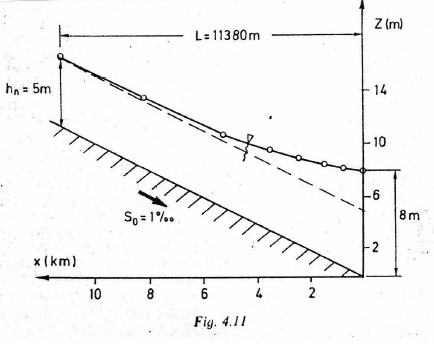
\includegraphics[height=2.5in]{bw_curve1.jpg} 
   \caption{Example backwater curve} 
   \label{fig:example1}
\end{figure}
\clearpage

\item A plan view of a rectangular channel of variable width as shown in Figure \ref{fig:NonPrismaticExample}.\\

\begin{figure}[h!] %  figure placement: here, top, bottom, or page
   \centering
   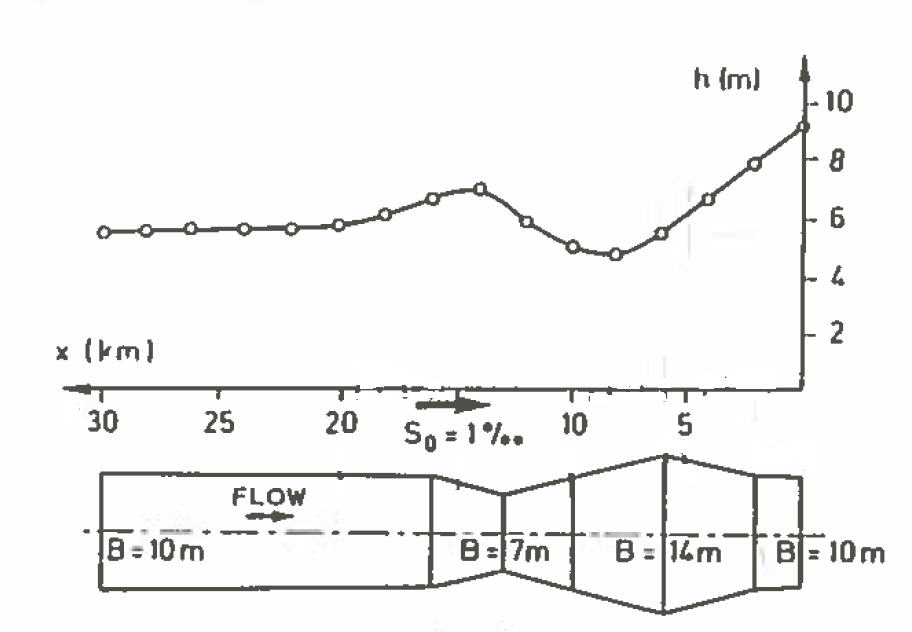
\includegraphics[width=2.5in]{NonPrismaticExample} 
   \caption{Non-Prismatic Rectangular Channel}
   \label{fig:NonPrismaticExample}
\end{figure}

The channel conveys $Q=100~m^3/sec$, with a bottom slope of $0.001$ and average Manning's $n$ value of $0.033$.  
A backwater curve is caused by a weir at the downstream end (to the right in the figure) by a 7 meter tall weir.
Flow depth over the weir is at critical depth $h_c = 2.17$ meters.  Start with the flow depth at normal depth and assume critical flow at the right boundary and observe if the transient solver will produce an equilibrium solution that is the same as the steady-flow solver.  

\item Analyze the flow in a 1000-m long trapezoidal channel with a bottom width of 20-m, side slope of 2H:1V, longitudinal slope S0=0.0001, and Manning's resistance n=0.013. Initial discharge in the channel is 110 m3/s and initial flow depth is 3.069 m. Simulate the flow and depth at every 100-m station when a downstream gate is closed at t=0. Produce a graph of depth and velocity versus location for t= 0, 60, 360 , 3600, 36,000 sec. (This is the same problem used in lecture)

\item Repeat the previous problem with the channel at equilibrium (no flow, the gate is closed).  Simulate the flow and depth at every 100-m station when the  downstream gate is opened at t=0\footnote{Boundary condition is a specified velocity -- can assume some function of critical depth when the gate is opened, document your assumption}. Produce a graph of depth and velocity versus location for t= 0, 60, 360 , 3600, 36,000 sec. 

\item The initial depth in a horizontal channel of rectangular cross section is 1 meter. 
The channel is 29 kilometers long and ends with a non-reflection boundary condition.
\newpage
\begin{figure}[h!] %  figure placement: here, top, bottom, or page
   \centering
   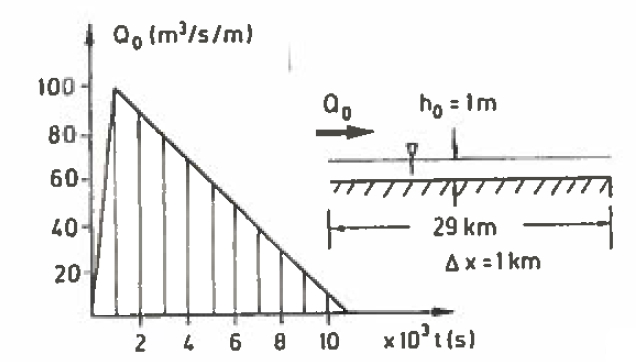
\includegraphics[width=4.25in]{upstreamHydro.jpg} 
   \caption{Upstream hydrograph for example}
   \label{fig:upstreamHydro}
\end{figure}

The initial discharge in the channel is 0 cubic meters per second. 
The upstream input hydrograph is shown in Figure \ref{fig:upstreamHydro}.
The manning friction factor is $n=1/40$.
Simulate the water surface elevation over time in the channel.\footnote{Example 4.1, Page 70. Koutitas, C.G. (1983). Elements of Computational Hydraulics. Pentech Press, London 138p. ISBN 0-7273-0503-4 }
\end{enumerate}

Save your results in addition to preparing the report -- you will rebuild all these models in \url{HEC-RAS} or \url{SWMM} to discover the similarity in results and have an understanding of what goes on under the hood in that professional program.
\end{document}  